\documentclass[12pt,a4paper,oneside, titlepage]{report}

\usepackage[utf8]{inputenc}
\usepackage[T1]{fontenc}
\usepackage[french]{babel}
\usepackage{amssymb}
\usepackage{amsmath}
\usepackage{graphicx}
\usepackage{float}
\usepackage{mathtools}
\usepackage[table,xcdraw]{xcolor}


\author{Matteo Besançon}

\title {Parallélisme \\ \large TP 5}
\date{\today}


\begin{document}

	\maketitle
	\newpage

	\section*{Introduction}

		Le but de ce TP est de réaliser une analyse des différentes stratégies de load balancing sur un algorithme.
		L'algorithme choisi est le calcul de l'ensemble de Julia. L'ensemble de Julia comprend tout les points $z$ représentés sur un plan complexe pour lesquels la suite :

		$$z_{n+1} = z^{2}_{n} + c$$

		ne diverge pas.

		Dans notre cas, nous nous concentrerons sur la portion du plan complexe $[-2, 2] \times [-2i, -2i] \in \mathbb{C}$

		L'un des gros avantages d'utiliser cet algorithme réside dans le fait qu'il s'agisse d'un algorithme complètement local, qui ne nécessite aucune communication.
		Grâce à cela, il est possible d'analyser les performances des différentes stratégies sans parasite.

		\subsection*{Répartition simple}
			Le but de la répartition simple est de diviser la matrice de façon équitable, c'est la stratégie que nous avions implémenté pour le TP4.
			Si on a une matrice $m \times n$ ou $m$ est la largeur et $n$ la hauteur de la matrice, alors on répartit les lignes de la matrice en sous-matrices de dimensions
			$\frac{n}{P}$ où $P$ est le nombre de processeurs ou de threads disponibles.

		\subsection*{Répartition statique}
			Dans la répartition statique, chaque processeur ou threads traite $\frac{n}{P}$ lignes, comme dans la répartition simple. Cependant, au lieu de prendre des blocs de lignes qui se suivent, on leur attribue des lignes à intervalle régulier.
			Pour un processeur d'indice $i$, on lui attribuera les lignes d'indice $j$ qui remplissent l'équation suivante $$j \equiv i \mathrm{mod} P$$
		\subsection*{Répartition Dynamique}
			Dans le processus de répartition dynamique, ce sont les threads ou les processeurs qui vont "chercher" les lignes à traiter, plutôt qu'un mécanisme externe qui les leur attribue.
			Baraquement, chaque thread va chercher un sous-domaine de taille arbitraire fixé, il le traite, puis va chercher un autre sous domaine. Chaque thread répète ces opérations jusqu'à ce qu'il ne reste plus de lignes à traiter dans le domaine principal.

			L'avantage principal de cette méthode est que, dans le cas ou pas tout les threads travaillent à la même vitesse, la plus lente ne ralentirons pas l'exécution totale de l'algorithme.
			Il faut cependant s'assurer que les threads ne s'attribuent pas le même sous domaine. Il faut donc prendre en compte l'exclusion mutuelle de la fonction d'attribution.

	\section*{Méthode}
		 Pour commencer, nous avons implémenté les trois stratégies de répartition de charge avec les threads et les stratégies simple et statique avec MPI.

		On a ensuite effectué des mesures de temps d'exécution en se concentrant sur l'exécution de l'algorithme de Julia (on ne mesure pas le temps d'exécution de l'image).

		Comme c'est la valeur de $c$ qui détermine la forme du fractal, on a commencé par choisir une valeur qui donnait une image intéressante. Nous avons décidé d'utiliser $c = 0.285 + 0.013\ i$.

		Les algorithmes ont étés exécutés respectivement avec 1, 2, 4, 8, 10, 12, 16 et 20 coeurs pour les threads et 1, 10, 20, 40, 60, 80, 100 et 120 coeurs avec MPI avec des matrices de hauteur 15'000 et de largeur 20'000 pour un total de maximum 5000 itérations.

Pour la stratégie Dynamique, nous avons également décidé d'exécuter l'algorithme avec des sous-domaines de hauteur 1, 10, 100, 1000 et 10'000.

	\newpage
	\section*{Résultats}

 		Afin de pouvoir intégrer une image d'exemple dans ce rapport nous avons exécuté l'algorithme trivial en local avec un domaine de 1500 par 2000 et un nombre maximum d'itération de 500.

		\begin{figure}[H]
			\centering
			
\includegraphics[scale=0.20]{images/julia_thread_simple}
			\caption {Image d'un fractal crée avec l'algorithme de Julia, converti en JPEG}
		\end{figure}

		\newpage

		 Les données dans les deux tableaux suivants correspondent aux mesures de temps, en $ms$. Toute l'agrégation des données et les graphes ont été réalisés grâce à un script python.

		\begin{table}[H]
			\centering
			\begin{tabular}{c|l|l|}
				\cline{2-3}
				\multicolumn{1}{l|}{}                                      & \multicolumn{2}{c|}{\textit{\textbf{MPI}}}                                                                                                                                \\ \hline
				\multicolumn{1}{|c|}{\textit{\textbf{CPUs}}}               & \multicolumn{1}{c|}{\cellcolor[HTML]{EFEFEF}{\color[HTML]{343434} \textbf{simple}}} & \multicolumn{1}{c|}{\cellcolor[HTML]{EFEFEF}{\color[HTML]{343434} \textbf{static}}} \\ \hline
				\multicolumn{1}{|c|}{\cellcolor[HTML]{EFEFEF}\textbf{1}}   & 774101.0                                                                            & 778724.0                                                                            \\ \hline
				\multicolumn{1}{|c|}{\cellcolor[HTML]{EFEFEF}\textbf{10}}  & 170399.0                                                                            & 164124.0                                                                            \\ \hline
				\multicolumn{1}{|c|}{\cellcolor[HTML]{EFEFEF}\textbf{20}}  & 86630.0                                                                             & 85999.0                                                                             \\ \hline
				\multicolumn{1}{|c|}{\cellcolor[HTML]{EFEFEF}\textbf{40}}  & 48037.0                                                                             & 45794.0                                                                             \\ \hline
				\multicolumn{1}{|c|}{\cellcolor[HTML]{EFEFEF}\textbf{60}}  & 31611.0                                                                             & 30255.0                                                                             \\ \hline
				\multicolumn{1}{|c|}{\cellcolor[HTML]{EFEFEF}\textbf{80}}  & 24711.0                                                                             & 21718.0                                                                             \\ \hline
				\multicolumn{1}{|c|}{\cellcolor[HTML]{EFEFEF}\textbf{100}} & 20076.0                                                                             & 20271.0                                                                             \\ \hline
				\multicolumn{1}{|c|}{\cellcolor[HTML]{EFEFEF}\textbf{120}} & 16871.0                                                                             & 19662.0                                                                             \\ \hline
			\end{tabular}
			\caption{Temps d'exécution des algorithmes MPI en ms}
		\end{table}


		\begin{table}[H]
			\centering
			\begin{tabular}{c|l|l|l|l|}
				\cline{2-5}
				\multicolumn{1}{l|}{}                                     & \multicolumn{4}{c|}{\textit{\textbf{Threads}}}                                                                                                                                                                                                                         \\ \hline
				\multicolumn{1}{|c|}{\textit{\textbf{CPUs}}}              & \multicolumn{1}{c|}{\cellcolor[HTML]{EFEFEF}\textbf{dynamic 100}} & \multicolumn{1}{c|}{\cellcolor[HTML]{EFEFEF}\textbf{dynamic 1000}} & \multicolumn{1}{c|}{\cellcolor[HTML]{EFEFEF}\textbf{simple}} & \multicolumn{1}{c|}{\cellcolor[HTML]{EFEFEF}\textbf{static}} \\ \hline
				\multicolumn{1}{|c|}{\cellcolor[HTML]{EFEFEF}\textbf{1}}  & 748343.0                                                           & 676615.0                                                            & 653636.0                                                     & 656872.0                                                     \\ \hline
				\multicolumn{1}{|c|}{\cellcolor[HTML]{EFEFEF}\textbf{2}}  & 393871.0                                                           & 369504.0                                                            & 356284.0                                                     & 401487.0                                                     \\ \hline
				\multicolumn{1}{|c|}{\cellcolor[HTML]{EFEFEF}\textbf{4}}  & 225568.0                                                           & 164927.0                                                            & 316261.0                                                     & 165678.0                                                     \\ \hline
				\multicolumn{1}{|c|}{\cellcolor[HTML]{EFEFEF}\textbf{8}}  & 144539.0                                                           & 134053.0                                                            & 166083.0                                                     & 135636.0                                                     \\ \hline
				\multicolumn{1}{|c|}{\cellcolor[HTML]{EFEFEF}\textbf{10}} & 129619.0                                                           & 126512.0                                                            & 162470.0                                                     & 71609.0                                                      \\ \hline
				\multicolumn{1}{|c|}{\cellcolor[HTML]{EFEFEF}\textbf{12}} & 124218.0                                                           & 99471.0                                                             & 148444.0                                                     & 78913.0                                                      \\ \hline
				\multicolumn{1}{|c|}{\cellcolor[HTML]{EFEFEF}\textbf{16}} & 103812.0                                                           & 83837.0                                                             & 88526.0                                                      & 41425.0                                                      \\ \hline
				\multicolumn{1}{|c|}{\cellcolor[HTML]{EFEFEF}\textbf{20}} & 105511.0                                                           & 82531.0                                                             & 77023.0                                                      & 40102.0                                                      \\ \hline
			\end{tabular}
			\caption{Temps d'exécution des algorithmes avec des threads en ms}
		\end{table}

		\newpage

		On compile ces données sur un graph représentant le temps d'exécution en fonction du nombre de CPUs.

		\begin{figure}[H]
			\centering
			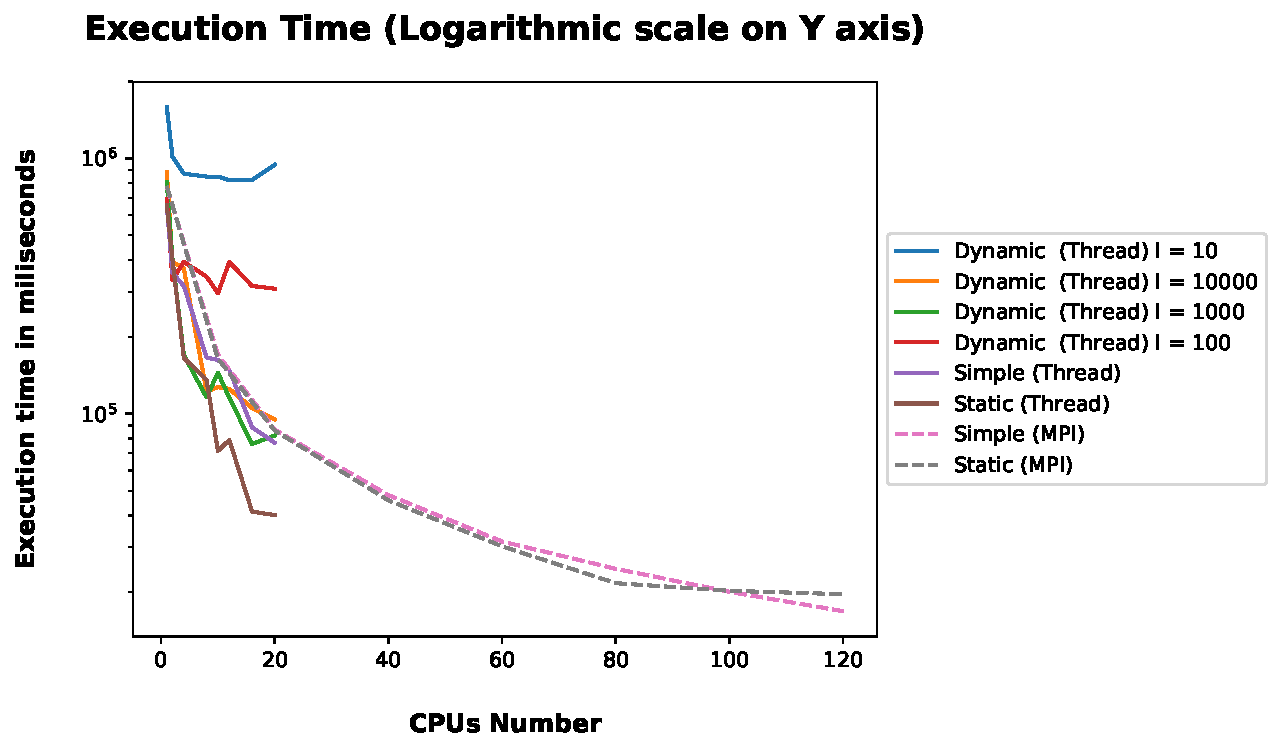
\includegraphics[scale=0.85]{graphs/execTime}
			\caption {Temps d'exécution de chaque algorithmes en ms}
		\end{figure}

		\newpage

		A partir de ces données brutes on peut calculer le speedup en utilisant les mêmes formules qu'au TP4.

		On a donc les données brutes suivantes :


		\begin{table}[H]
			\centering
			\begin{tabular}{c|l|l|}
				\cline{2-3}
				\multicolumn{1}{l|}{}                                      & \multicolumn{2}{c|}{\textit{\textbf{MPI}}}                                                                                  \\ \hline
				\multicolumn{1}{|c|}{\textit{\textbf{CPUs}}}               & \multicolumn{1}{c|}{\cellcolor[HTML]{EFEFEF}\textbf{simple}} & \multicolumn{1}{c|}{\cellcolor[HTML]{EFEFEF}\textbf{static}} \\ \hline
				\multicolumn{1}{|c|}{\cellcolor[HTML]{EFEFEF}\textbf{1}}   & 1.0                                                          & 1.0                                                          \\ \hline
				\multicolumn{1}{|c|}{\cellcolor[HTML]{EFEFEF}\textbf{10}}  & 4.54287290418371                                             & 4.744729594696692                                            \\ \hline
				\multicolumn{1}{|c|}{\cellcolor[HTML]{EFEFEF}\textbf{20}}  & 8.935715110238947                                            & 9.055035523668879                                            \\ \hline
				\multicolumn{1}{|c|}{\cellcolor[HTML]{EFEFEF}\textbf{40}}  & 16.114682432291776                                           & 17.004935144342053                                           \\ \hline
				\multicolumn{1}{|c|}{\cellcolor[HTML]{EFEFEF}\textbf{60}}  & 24.488342665527824                                           & 25.738687820195008                                           \\ \hline
				\multicolumn{1}{|c|}{\cellcolor[HTML]{EFEFEF}\textbf{80}}  & 31.326170531342317                                           & 35.85615618381066                                            \\ \hline
				\multicolumn{1}{|c|}{\cellcolor[HTML]{EFEFEF}\textbf{100}} & 38.55852759513847                                            & 38.41566770262937                                            \\ \hline
				\multicolumn{1}{|c|}{\cellcolor[HTML]{EFEFEF}\textbf{120}} & 45.8835279473653                                             & 39.60553351642763                                            \\ \hline
			\end{tabular}
			\caption{Données brutes du speedup des algorithmes MPI}
		\end{table}

		Ce qui nous donne :

		\begin{figure}[H]
			\centering
			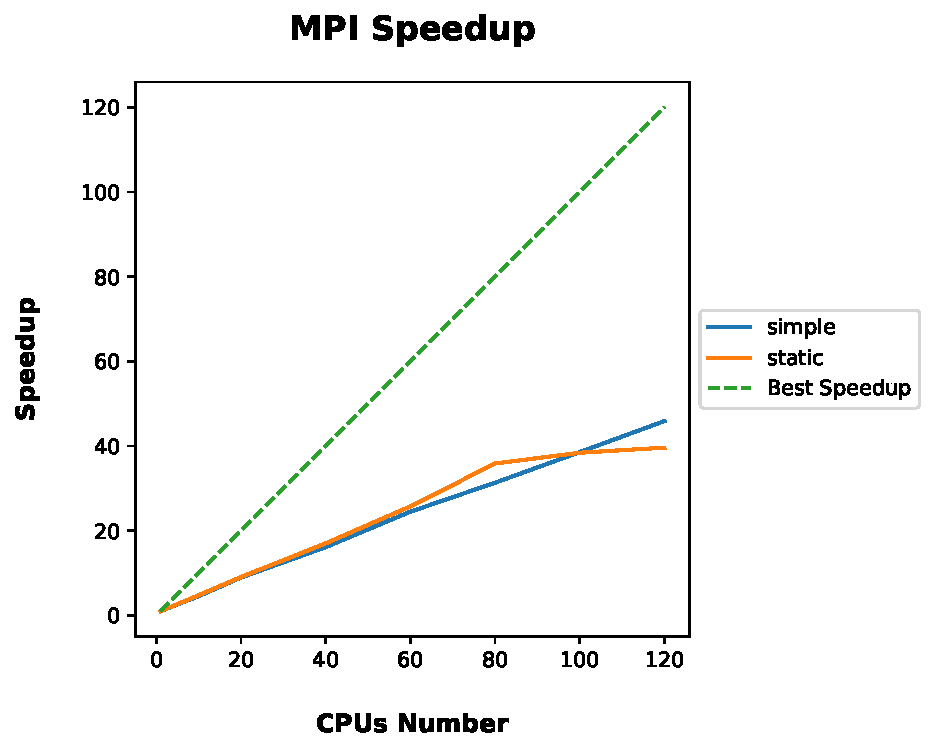
\includegraphics[scale=0.80]{graphs/speedupMPI}
			\caption {Speedup des algorithmes MPI}
		\end{figure}


		\begin{table}[H]
			\centering
			\resizebox{\textwidth}{!}{\begin{tabular}{c|l|l|l|l|}
				\cline{2-5}
				\multicolumn{1}{l|}{}                                     & \multicolumn{4}{c|}{\textit{\textbf{Threads}}}                                                                                                                                                                                                                       \\ \hline
				\multicolumn{1}{|c|}{\textit{\textbf{CPUs Number}}}       & \multicolumn{1}{c|}{\cellcolor[HTML]{EFEFEF}\textbf{dynamic 100}} & \multicolumn{1}{c|}{\cellcolor[HTML]{EFEFEF}\textbf{dynamic 1000}} & \multicolumn{1}{c|}{\cellcolor[HTML]{EFEFEF}\textbf{static}} & \multicolumn{1}{c|}{\cellcolor[HTML]{EFEFEF}\textbf{simple}} \\ \hline
				\multicolumn{1}{|c|}{\cellcolor[HTML]{EFEFEF}\textbf{1}}  & 1.0                                                               & 1.0                                                                & 1.0                                                          & 1.0                                                          \\ \hline
				\multicolumn{1}{|c|}{\cellcolor[HTML]{EFEFEF}\textbf{2}}  & 1.8999697870622616                                                & 1.8311439118385728                                                 & 1.6360978064046905                                           & 1.8345926283526626                                           \\ \hline
				\multicolumn{1}{|c|}{\cellcolor[HTML]{EFEFEF}\textbf{4}}  & 3.317593807632288                                                 & 4.102512020469662                                                  & 3.9647509023527565                                           & 2.0667613142309675                                           \\ \hline
				\multicolumn{1}{|c|}{\cellcolor[HTML]{EFEFEF}\textbf{8}}  & 5.177446917440967                                                 & 5.047369324073315                                                  & 4.8429030640832815                                           & 3.935598465827327                                            \\ \hline
				\multicolumn{1}{|c|}{\cellcolor[HTML]{EFEFEF}\textbf{10}} & 5.773405133506662                                                 & 5.348227836094599                                                  & 9.17303690876845                                             & 4.023118114113375                                            \\ \hline
				\multicolumn{1}{|c|}{\cellcolor[HTML]{EFEFEF}\textbf{12}} & 6.024432851921621                                                 & 6.802133285078063                                                  & 8.324002382370459                                            & 4.403249710328474                                            \\ \hline
				\multicolumn{1}{|c|}{\cellcolor[HTML]{EFEFEF}\textbf{16}} & 7.208636766462451                                                 & 8.070601285828452                                                  & 15.856898008449004                                           & 7.383548336082055                                            \\ \hline
				\multicolumn{1}{|c|}{\cellcolor[HTML]{EFEFEF}\textbf{20}} & 7.092559069670461                                                 & 8.198313361040094                                                  & 16.380030921151064                                           & 8.486244368565234                                            \\ \hline
			\end{tabular}}
			\caption{Données brutes du speedup des algorithmes threads}
		\end{table}


		\begin{figure}[H]
			\centering
			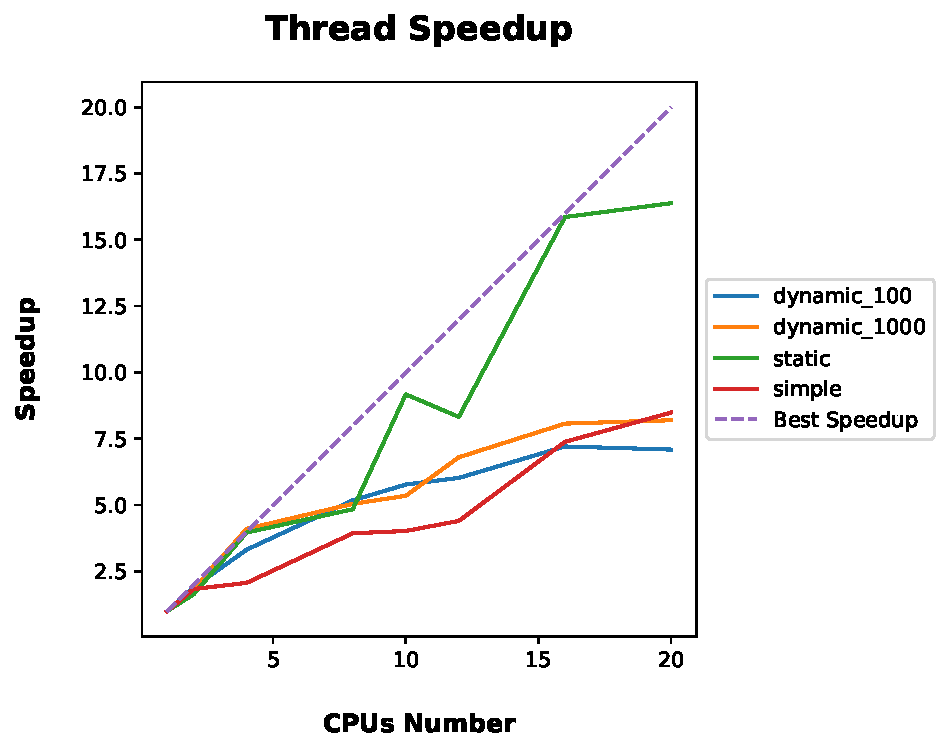
\includegraphics[scale=0.80]{graphs/speedupThread}
			\caption {Speedup des algorithmes threads}
		\end{figure}

		\newpage

	\section*{Conclusion}

		En regardant les résultats présentés dans la section précédente, la première chose que l'on peut remarquer, c'est que pour les mêmes stratégies de load balancing, les implémentations utilisant des threads sont sensiblement plus rapides.
		Cette différence est principalement due au calcul de la divergence. En effet, dans une implémentation avec des threads, la matrice est partagée entre chaque thread, chaque thread a la vision globale de la matrice. Alors que dans l'implémentation MPI, la fonction Julia travaille toujours sur un sous-domaine sans avoir la "vision d'ensemble" du reste du domaine. Il devient donc nécessaire de projeter le plan complexe sur le domaine, ce qui rajoute un nombre comparable d'opérations, surtout pour l'implémentation statique.

		En regardant le graphe des temps d'exécution ainsi que celui du speedup que dans notre cas la répartition statique avec les threads est la plus performante. Cependant, la répartition dynamique est à peine plus lentes avec peu de CPU et que l'écart se creuse en augmentant le nombre de CPU.
		Ceci pourrait être du au choix de $l$ qui a été fait. En effet, la taille du sous-domaine corrèlée avec le nombre de CPU influencent sur les performances.

		J'ai par exemple effectué un test (pas représenté dans les tableaux pour des raisons de lisibilité, mais les données, sont visibles sur les graphes) avec un sous-domaine ayant une hauteur de 10'000 et l'on remarque qu'à partir de 2 CPU le temps d'exécution stagne. En effet, avec cette stratégie d'allocation, seuls deux CPUs peuvent être utilisés pour ces valeurs (domaines de 15'000 et sous-domaine de 10'000).

		Dans la même idée, en choisissant un l trop petit, les threads effectuent rapidement le calcul pour leur sous-domaine, par contre, comme la fonction d'attribution d'un nouveau sous-domaine est en exclusion mutuelle, ils passeront beaucoup de temps à attendre pour pouvoir exécuter cette dernière. J'avais effectué un test avec l=1, cependant, en raison du temps d'exécution trop élevé, je n'ai pas pu obtenir de résultats utilisables.

		Si je devais refaire ce travail, je prendrais beaucoup plus de mesure pour chaque paramètres, de cette façon, il serait possible de faire une moyenne des résultats pour obtenir des graphes un peu plus précis.




\end{document}
